\documentclass{homeworg}
\usepackage{enumitem}
\usepackage{listings}
\usepackage{color} %red, green, blue, yellow, cyan, magenta, black, white
\definecolor{mygreen}{RGB}{28,172,0} % color values Red, Green, Blue
\definecolor{mylilas}{RGB}{170,55,241}
\usepackage{xcolor,cancel}
% --------------- GRAPHIC PACKAGES ----------------------------
\usepackage{graphicx}
\graphicspath{{./images/}}
\usepackage{wrapfig}
% --------------- HCANCEL COMMAND -----------------------------
\newcommand\hcancel[2][black]{\setbox0=\hbox{$#2$}%
\rlap{\raisebox{.45\ht0}{\textcolor{#1}{\rule{\wd0}{1pt}}}}#2}

% --------------- TRANSPOSE COMMAND -----------------------------
\newcommand{\transpose}[1]{\ensuremath{#1^{\scriptscriptstyle T}}}


\begin{document}

% --------------- MATLAB Code settings -----------------------
\lstset{language=Matlab,%
    %basicstyle=\color{red},
    breaklines=true,%
    morekeywords={matlab2tikz},
    keywordstyle=\color{blue},%
    morekeywords=[2]{1}, keywordstyle=[2]{\color{black}},
    identifierstyle=\color{black},%
    stringstyle=\color{mylilas},
    commentstyle=\color{mygreen},%
    showstringspaces=false,%without this there will be a symbol in the places where there is a space
    numbers=left,%
    numberstyle={\tiny \color{black}},% size of the numbers
    numbersep=9pt, % this defines how far the numbers are from the text
    emph=[1]{for,end,break},emphstyle=[1]\color{red}, %some words to emphasise
    %emph=[2]{word1,word2}, emphstyle=[2]{style},
}

% --------------- Title -------------------------------------
%\maketitle
\begin{center}
\textbf{EE 5323 - HW05}\\
\end{center}

\noindent
Bardia Mojra\\
1000766739\\
\today\\
HW05 -- Lyapunov Stability Analysis \\
EE 5323 -- Nonlinear Systems\\
Dr. Frank Lewis

\exercise
\noindent
\textbf{Lyapunov's Direct Method - SISL}\\
Consider the system
\begin{equation*}
  \begin{cases}
    \dot{x}_1 = x_1 x_2^2 - x_1\\
    \dot{x}_2 = -x_1^2 x_2\\
  \end{cases}
\end{equation*}
Use Lyapunov to study the stability. SISL? AS?\\

\noindent
\textbf{Answer} \\
1) Lyapunov function candidate: \( V(x_1, x_2) = \frac{1}{2} (x_1^2 + x_2^2) > 0\)
\begin{equation*}
\dot{V} = \frac{\partial V^\top}{\partial x} \dot{x} =\\
\begin{bmatrix}
\frac{\partial V}{\partial x_1} & \frac{\partial V}{\partial x_2}
\end{bmatrix}
\begin{bmatrix}
\dot{x}_1 \\
\dot{x}_2
\end{bmatrix}
=
\begin{bmatrix}
  x_1 & x_2
  \end{bmatrix}
  \begin{bmatrix}
  \dot{x}_1 \\
  \dot{x}_2
  \end{bmatrix}
  \Rightarrow
\end{equation*}
\begin{equation*}
\dot{V} =
  x_1 \dot{x}_1 + x_2 \dot{x}_2
\end{equation*}
Now we plug in system dynamics to check stability,
\begin{equation*}
  \dot{V} = x_1 (x_1 x_2^2 - x_1) + x_2(-x_1^2 x_2) \Rightarrow \\
\end{equation*}
\begin{equation*}
  \dot{V} = \hcancel[red]{x_1^2 x_2^2} - x_1^2 - \hcancel[red]{x_1^2 x_2^2}
\end{equation*}
\begin{equation*}
  \dot{V} = - x_1^2 \leq 0
\end{equation*}
Thus, the system is \emph{marginally stable} and it is considered \emph{SISL}.

\exercise
\noindent
\textbf{Lyapunov's Direct Method - AS}\\
Consider the system
\begin{equation*}
  \begin{cases}
    \dot{x}_1 = x_1 x_2^2 - x_1\\
    \dot{x}_2 = -x_1^2 x_2 - x_2\\
  \end{cases}
\end{equation*}

Use Lyapunov to study the stability. SISL? AS?

\noindent
\textbf{Answer} \\
2) Lyapunov function candidate: \( V(x_1, x_2) = \frac{1}{2} (x_1^2 + x_2^2) > 0\)
\begin{equation*}
\dot{V} = \frac{\partial V^\top}{\partial x} \dot{x} =\\
\begin{bmatrix}
\frac{\partial V}{\partial x_1} & \frac{\partial V}{\partial x_2}
\end{bmatrix}
\begin{bmatrix}
\dot{x}_1 \\
\dot{x}_2
\end{bmatrix}
=
\begin{bmatrix}
  x_1 & x_2
  \end{bmatrix}
  \begin{bmatrix}
  \dot{x}_1 \\
  \dot{x}_2
  \end{bmatrix}
  \Rightarrow
\end{equation*}
\begin{equation*}
\dot{V} =
  x_1 \dot{x}_1 + x_2 \dot{x}_2
\end{equation*}
Now we plug in system dynamics to check stability,
\begin{equation*}
  \dot{V} = x_1 (x_1 x_2^2 - x_1) + x_2(-x_1^2 x_2 - x_2) \Rightarrow
\end{equation*}
\begin{equation*}
  \dot{V} = \hcancel[red]{x_1^2 x_2^2} - x_1^2 - \hcancel[red]{x_1^2 x_2^2} - x_2^2
\end{equation*}
\begin{equation*}
  \dot{V} = - x_1^2 - x_2^2 < 0
\end{equation*}
Thus, the system is \emph{asymptotically stable} (AS). Moreover, one can assume
it is \emph{global asymptotically stable} (GAS) since the Lyapunov function is
always \underline{negative}.


\exercise
\noindent
\textbf{Asymptotic Stability Simulation}\\
a) Use Lyapunov to show that the system
\begin{equation*}
  \begin{cases}
    \dot{x}_1 = x_1 x_2^2 - x_1 (x_1^2 + x_2^2 -3)\\
    \dot{x}_2 = -x_1^2 x_2 - x_2(x_1^2 + x_2^2 -3)\\
  \end{cases}
\end{equation*}
is locally asymptotically stable. Find the Region of Asymptotic Stability.\\
b) Simulate the system from many uniformly spaced ICs.

\noindent
\textbf{Answer} \\
3.a) Lyapunov function candidate: \( V(x_1, x_2) = \frac{1}{2} (x_1^2 + x_2^2) > 0\)
\begin{equation*}
\dot{V} = \frac{\partial V^\top}{\partial x} \dot{x} =
\begin{bmatrix}
\frac{\partial V}{\partial x_1} & \frac{\partial V}{\partial x_2}
\end{bmatrix}
\begin{bmatrix}
\dot{x}_1 \\
\dot{x}_2
\end{bmatrix}
=
\begin{bmatrix}
  x_1 & x_2
  \end{bmatrix}
  \begin{bmatrix}
  \dot{x}_1 \\
  \dot{x}_2
  \end{bmatrix}
  \Rightarrow
\end{equation*}
\begin{equation*}
\dot{V} =
  x_1 \dot{x}_1 + x_2 \dot{x}_2
\end{equation*}
Now we plug in system dynamics to check stability,
\begin{equation*}
  \dot{V} = x_1 (x_1 x_2^2 - x_1 (x_1^2 + x_2^2 -3)) + x_2(-x_1^2 x_2 - x_2(x_1^2 + x_2^2 -3)) \Rightarrow
\end{equation*}
\begin{equation*}
  \dot{V} = \hcancel[red]{x_1^2 x_2^2} - x_1^2(x_1^2 + x_2^2 -3) - \hcancel[red]{x_1^2 x_2^2} - x_2^2(x_1^2 + x_2^2 -3)
\end{equation*}
\begin{equation*}
  \dot{V} = (x_1^2 + x_2^2 -3)(- x_1^2 - x_2^2) < 0
\end{equation*}
Thus, the system is \emph{asymptotically stable} (AS) and it is bound by a region
with radius of \(\sqrt{3}\).

3.b) Simulation:
\begin{figure}[h]
  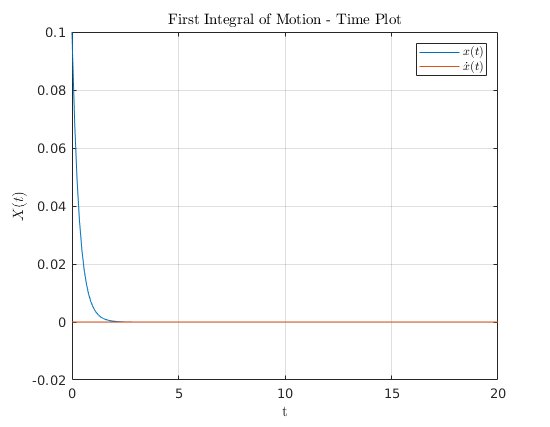
\includegraphics[width=.6\textwidth]{fig01.png}
  \centering
\end{figure}
\begin{figure}[h]
  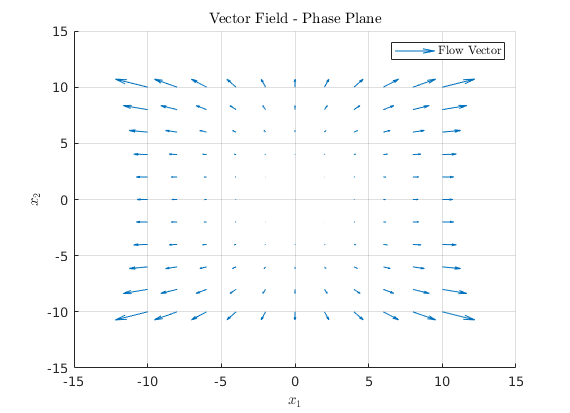
\includegraphics[width=.6\textwidth]{fig02.png}
  \centering
\end{figure}
\begin{figure}[h]
  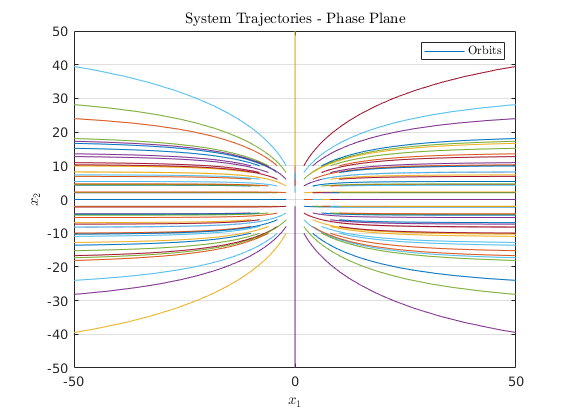
\includegraphics[width=.6\textwidth]{fig03.png}
  \centering
\end{figure}
\newpage
\noindent
\textbf{Matlab Code}\\
\lstinputlisting{hw05_q03_code.m}



\exercise
\noindent
\textbf{SISL Simulation}\\
a) Use quadratic Lyapunov Function to show this system is locally SISL
\begin{equation*}
  \begin{cases}
    \dot{x}_1 = x_2 + x_1 (x_1^2 -2)\\
    \dot{x}_2 = -x_1\\
  \end{cases}
\end{equation*}
Find a region within which \(V \leq 0\).\\
b) Simulate the system from many uniformly spaced ICs.

\noindent
\textbf{Answer} \\
4.a) Lyapunov function candidate: \( V(x_1, x_2) = \frac{1}{2} (x_1^2 + x_2^2) > 0\)
\begin{equation*}
\dot{V} = \frac{\partial V^\top}{\partial x} \dot{x} =
\begin{bmatrix}
\frac{\partial V}{\partial x_1} & \frac{\partial V}{\partial x_2}
\end{bmatrix}
\begin{bmatrix}
\dot{x}_1 \\
\dot{x}_2
\end{bmatrix}
=
\begin{bmatrix}
  x_1 & x_2
  \end{bmatrix}
  \begin{bmatrix}
  \dot{x}_1 \\
  \dot{x}_2
  \end{bmatrix}
  \Rightarrow
\end{equation*}
\begin{equation*}
\dot{V} =
  x_1 \dot{x}_1 + x_2 \dot{x}_2
\end{equation*}
Now we plug in system dynamics to check stability,
\begin{equation*}
  \dot{V} = x_1 (x_2 + x_1 (x_1^2 -2)) + x_2(-x_1) \Rightarrow
\end{equation*}
\begin{equation*}
  \dot{V} = \hcancel[red]{x_1 x_2} - x_1^2(x_1^2 -2) - \hcancel[red]{x_1 x_2}
\end{equation*}
\begin{equation*}
  \dot{V} = - x_1^2(x_1^2 -2) \leq 0
\end{equation*}
Thus, the system is \emph{asymptotically stable} (AS) and it is bound by a region
with radius of \(\sqrt{3}\).

4.b) Simulation:
\begin{figure}[h]
  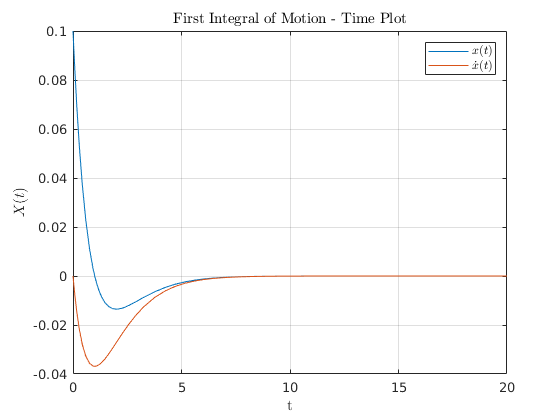
\includegraphics[width=.6\textwidth]{fig04.png}
  \centering
\end{figure}
\begin{figure}[h]
  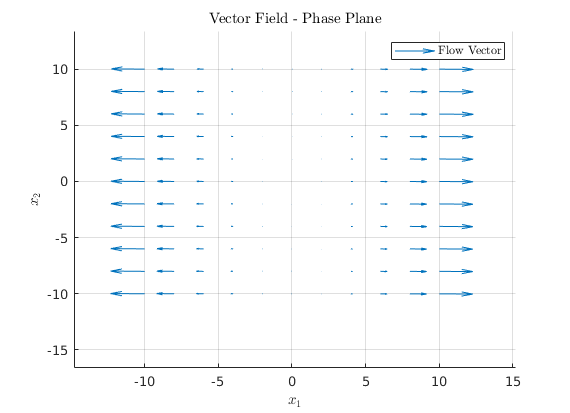
\includegraphics[width=.6\textwidth]{fig05.png}
  \centering
\end{figure}
\begin{figure}[h]
  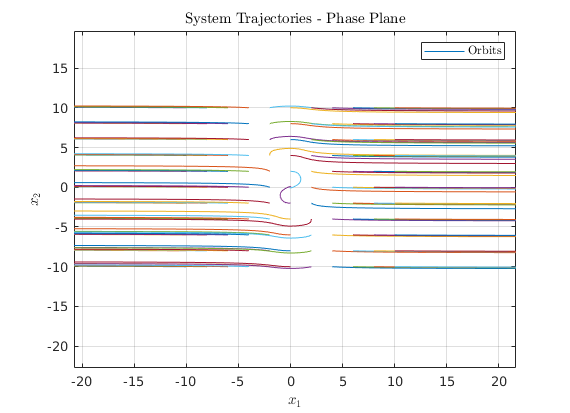
\includegraphics[width=.6\textwidth]{fig06.png}
  \centering
\end{figure}
\newpage
\noindent
\textbf{Matlab Code}\\
\lstinputlisting{hw05_q04_code.m}
%\bibliography{ref}

\end{document}
